% Options for packages loaded elsewhere
\PassOptionsToPackage{unicode}{hyperref}
\PassOptionsToPackage{hyphens}{url}
%
\documentclass[
  11pt,
  letterpaper,
]{scrbook}

\usepackage{amsmath,amssymb}
\usepackage{iftex}
\ifPDFTeX
  \usepackage[T1]{fontenc}
  \usepackage[utf8]{inputenc}
  \usepackage{textcomp} % provide euro and other symbols
\else % if luatex or xetex
  \usepackage{unicode-math}
  \defaultfontfeatures{Scale=MatchLowercase}
  \defaultfontfeatures[\rmfamily]{Ligatures=TeX,Scale=1}
\fi
\usepackage{lmodern}
\ifPDFTeX\else  
    % xetex/luatex font selection
\fi
% Use upquote if available, for straight quotes in verbatim environments
\IfFileExists{upquote.sty}{\usepackage{upquote}}{}
\IfFileExists{microtype.sty}{% use microtype if available
  \usepackage[]{microtype}
  \UseMicrotypeSet[protrusion]{basicmath} % disable protrusion for tt fonts
}{}
\makeatletter
\@ifundefined{KOMAClassName}{% if non-KOMA class
  \IfFileExists{parskip.sty}{%
    \usepackage{parskip}
  }{% else
    \setlength{\parindent}{0pt}
    \setlength{\parskip}{6pt plus 2pt minus 1pt}}
}{% if KOMA class
  \KOMAoptions{parskip=half}}
\makeatother
\usepackage{xcolor}
\setlength{\emergencystretch}{3em} % prevent overfull lines
\setcounter{secnumdepth}{5}
% Make \paragraph and \subparagraph free-standing
\ifx\paragraph\undefined\else
  \let\oldparagraph\paragraph
  \renewcommand{\paragraph}[1]{\oldparagraph{#1}\mbox{}}
\fi
\ifx\subparagraph\undefined\else
  \let\oldsubparagraph\subparagraph
  \renewcommand{\subparagraph}[1]{\oldsubparagraph{#1}\mbox{}}
\fi

\usepackage{color}
\usepackage{fancyvrb}
\newcommand{\VerbBar}{|}
\newcommand{\VERB}{\Verb[commandchars=\\\{\}]}
\DefineVerbatimEnvironment{Highlighting}{Verbatim}{commandchars=\\\{\}}
% Add ',fontsize=\small' for more characters per line
\usepackage{framed}
\definecolor{shadecolor}{RGB}{241,243,245}
\newenvironment{Shaded}{\begin{snugshade}}{\end{snugshade}}
\newcommand{\AlertTok}[1]{\textcolor[rgb]{0.68,0.00,0.00}{#1}}
\newcommand{\AnnotationTok}[1]{\textcolor[rgb]{0.37,0.37,0.37}{#1}}
\newcommand{\AttributeTok}[1]{\textcolor[rgb]{0.40,0.45,0.13}{#1}}
\newcommand{\BaseNTok}[1]{\textcolor[rgb]{0.68,0.00,0.00}{#1}}
\newcommand{\BuiltInTok}[1]{\textcolor[rgb]{0.00,0.23,0.31}{#1}}
\newcommand{\CharTok}[1]{\textcolor[rgb]{0.13,0.47,0.30}{#1}}
\newcommand{\CommentTok}[1]{\textcolor[rgb]{0.37,0.37,0.37}{#1}}
\newcommand{\CommentVarTok}[1]{\textcolor[rgb]{0.37,0.37,0.37}{\textit{#1}}}
\newcommand{\ConstantTok}[1]{\textcolor[rgb]{0.56,0.35,0.01}{#1}}
\newcommand{\ControlFlowTok}[1]{\textcolor[rgb]{0.00,0.23,0.31}{#1}}
\newcommand{\DataTypeTok}[1]{\textcolor[rgb]{0.68,0.00,0.00}{#1}}
\newcommand{\DecValTok}[1]{\textcolor[rgb]{0.68,0.00,0.00}{#1}}
\newcommand{\DocumentationTok}[1]{\textcolor[rgb]{0.37,0.37,0.37}{\textit{#1}}}
\newcommand{\ErrorTok}[1]{\textcolor[rgb]{0.68,0.00,0.00}{#1}}
\newcommand{\ExtensionTok}[1]{\textcolor[rgb]{0.00,0.23,0.31}{#1}}
\newcommand{\FloatTok}[1]{\textcolor[rgb]{0.68,0.00,0.00}{#1}}
\newcommand{\FunctionTok}[1]{\textcolor[rgb]{0.28,0.35,0.67}{#1}}
\newcommand{\ImportTok}[1]{\textcolor[rgb]{0.00,0.46,0.62}{#1}}
\newcommand{\InformationTok}[1]{\textcolor[rgb]{0.37,0.37,0.37}{#1}}
\newcommand{\KeywordTok}[1]{\textcolor[rgb]{0.00,0.23,0.31}{#1}}
\newcommand{\NormalTok}[1]{\textcolor[rgb]{0.00,0.23,0.31}{#1}}
\newcommand{\OperatorTok}[1]{\textcolor[rgb]{0.37,0.37,0.37}{#1}}
\newcommand{\OtherTok}[1]{\textcolor[rgb]{0.00,0.23,0.31}{#1}}
\newcommand{\PreprocessorTok}[1]{\textcolor[rgb]{0.68,0.00,0.00}{#1}}
\newcommand{\RegionMarkerTok}[1]{\textcolor[rgb]{0.00,0.23,0.31}{#1}}
\newcommand{\SpecialCharTok}[1]{\textcolor[rgb]{0.37,0.37,0.37}{#1}}
\newcommand{\SpecialStringTok}[1]{\textcolor[rgb]{0.13,0.47,0.30}{#1}}
\newcommand{\StringTok}[1]{\textcolor[rgb]{0.13,0.47,0.30}{#1}}
\newcommand{\VariableTok}[1]{\textcolor[rgb]{0.07,0.07,0.07}{#1}}
\newcommand{\VerbatimStringTok}[1]{\textcolor[rgb]{0.13,0.47,0.30}{#1}}
\newcommand{\WarningTok}[1]{\textcolor[rgb]{0.37,0.37,0.37}{\textit{#1}}}

\providecommand{\tightlist}{%
  \setlength{\itemsep}{0pt}\setlength{\parskip}{0pt}}\usepackage{longtable,booktabs,array}
\usepackage{calc} % for calculating minipage widths
% Correct order of tables after \paragraph or \subparagraph
\usepackage{etoolbox}
\makeatletter
\patchcmd\longtable{\par}{\if@noskipsec\mbox{}\fi\par}{}{}
\makeatother
% Allow footnotes in longtable head/foot
\IfFileExists{footnotehyper.sty}{\usepackage{footnotehyper}}{\usepackage{footnote}}
\makesavenoteenv{longtable}
\usepackage{graphicx}
\makeatletter
\def\maxwidth{\ifdim\Gin@nat@width>\linewidth\linewidth\else\Gin@nat@width\fi}
\def\maxheight{\ifdim\Gin@nat@height>\textheight\textheight\else\Gin@nat@height\fi}
\makeatother
% Scale images if necessary, so that they will not overflow the page
% margins by default, and it is still possible to overwrite the defaults
% using explicit options in \includegraphics[width, height, ...]{}
\setkeys{Gin}{width=\maxwidth,height=\maxheight,keepaspectratio}
% Set default figure placement to htbp
\makeatletter
\def\fps@figure{htbp}
\makeatother
\newlength{\cslhangindent}
\setlength{\cslhangindent}{1.5em}
\newlength{\csllabelwidth}
\setlength{\csllabelwidth}{3em}
\newlength{\cslentryspacingunit} % times entry-spacing
\setlength{\cslentryspacingunit}{\parskip}
\newenvironment{CSLReferences}[2] % #1 hanging-ident, #2 entry spacing
 {% don't indent paragraphs
  \setlength{\parindent}{0pt}
  % turn on hanging indent if param 1 is 1
  \ifodd #1
  \let\oldpar\par
  \def\par{\hangindent=\cslhangindent\oldpar}
  \fi
  % set entry spacing
  \setlength{\parskip}{#2\cslentryspacingunit}
 }%
 {}
\usepackage{calc}
\newcommand{\CSLBlock}[1]{#1\hfill\break}
\newcommand{\CSLLeftMargin}[1]{\parbox[t]{\csllabelwidth}{#1}}
\newcommand{\CSLRightInline}[1]{\parbox[t]{\linewidth - \csllabelwidth}{#1}\break}
\newcommand{\CSLIndent}[1]{\hspace{\cslhangindent}#1}

% \usepackage{amsmath,amssymb,mathtools}
\usepackage{mathtools}
\usepackage{enumerate}
\usepackage{geometry}
\geometry{hmargin=1.2in}

\usepackage{booktabs}
\usepackage{amssymb}
\makeatletter
\def\thm@space@setup{%
  \thm@preskip=8pt plus 2pt minus 4pt
  \thm@postskip=\thm@preskip
}
\makeatother

\usepackage{framed,color}
\definecolor{shadecolor}{RGB}{248,248,248}

\renewcommand{\textfraction}{0.05}
\renewcommand{\topfraction}{0.8}
\renewcommand{\bottomfraction}{0.8}
\renewcommand{\floatpagefraction}{0.75}

%\let\oldhref\href
%\renewcommand{\href}[2]{#2\footnote{\url{#1}}}

\ifxetex
  \usepackage{letltxmacro}
  \setlength{\XeTeXLinkMargin}{1pt}
  \LetLtxMacro\SavedIncludeGraphics\includegraphics
  \def\includegraphics#1#{% #1 catches optional stuff (star/opt. arg.)
    \IncludeGraphicsAux{#1}%
  }%
  \newcommand*{\IncludeGraphicsAux}[2]{%
    \XeTeXLinkBox{%
      \SavedIncludeGraphics#1{#2}%
    }%
  }%
\fi

\makeatletter
\newenvironment{kframe}{%
\medskip{}
\setlength{\fboxsep}{.8em}
 \def\at@end@of@kframe{}%
 \ifinner\ifhmode%
  \def\at@end@of@kframe{\end{minipage}}%
  \begin{minipage}{\columnwidth}%
 \fi\fi%
 \def\FrameCommand##1{\hskip\@totalleftmargin \hskip-\fboxsep
 \colorbox{shadecolor}{##1}\hskip-\fboxsep
     % There is no \\@totalrightmargin, so:
     \hskip-\linewidth \hskip-\@totalleftmargin \hskip\columnwidth}%
 \MakeFramed {\advance\hsize-\width
   \@totalleftmargin\z@ \linewidth\hsize
   \@setminipage}}%
 {\par\unskip\endMakeFramed%
 \at@end@of@kframe}
\makeatother

\makeatletter
\@ifundefined{Shaded}{
}{\renewenvironment{Shaded}{\begin{kframe}}{\end{kframe}}}
\makeatother

\newenvironment{rmdblock}[1]
  {
  \begin{itemize}
  \renewcommand{\labelitemi}{
    \raisebox{-.7\height}[0pt][0pt]{
      {\setkeys{Gin}{width=3em,keepaspectratio}\includegraphics{images/#1}}
    }
  }
  \setlength{\fboxsep}{1em}
  \begin{kframe}
  \item
  }
  {
  \end{kframe}
  \end{itemize}
  }
\newenvironment{rmdnote}
  {\begin{rmdblock}{note}}
  {\end{rmdblock}}
\newenvironment{rmdcaution}
  {\begin{rmdblock}{caution}}
  {\end{rmdblock}}
\newenvironment{rmdimportant}
  {\begin{rmdblock}{important}}
  {\end{rmdblock}}
\newenvironment{rmdtip}
  {\begin{rmdblock}{tip}}
  {\end{rmdblock}}
\newenvironment{rmdwarning}
  {\begin{rmdblock}{warning}}
  {\end{rmdblock}}
\usepackage{mathrsfs}
\DeclareMathAlphabet{\mathcrl}{U}{rsfs}{m}{n}
\usepackage{utopia}
\DeclareMathAlphabet{\mathcal}{OMS}{cmsy}{m}{n}
\makeatletter
\makeatother
\makeatletter
\@ifpackageloaded{bookmark}{}{\usepackage{bookmark}}
\makeatother
\makeatletter
\@ifpackageloaded{caption}{}{\usepackage{caption}}
\AtBeginDocument{%
\ifdefined\contentsname
  \renewcommand*\contentsname{Table of contents}
\else
  \newcommand\contentsname{Table of contents}
\fi
\ifdefined\listfigurename
  \renewcommand*\listfigurename{List of Figures}
\else
  \newcommand\listfigurename{List of Figures}
\fi
\ifdefined\listtablename
  \renewcommand*\listtablename{List of Tables}
\else
  \newcommand\listtablename{List of Tables}
\fi
\ifdefined\figurename
  \renewcommand*\figurename{Figure}
\else
  \newcommand\figurename{Figure}
\fi
\ifdefined\tablename
  \renewcommand*\tablename{Table}
\else
  \newcommand\tablename{Table}
\fi
}
\@ifpackageloaded{float}{}{\usepackage{float}}
\floatstyle{ruled}
\@ifundefined{c@chapter}{\newfloat{codelisting}{h}{lop}}{\newfloat{codelisting}{h}{lop}[chapter]}
\floatname{codelisting}{Listing}
\newcommand*\listoflistings{\listof{codelisting}{List of Listings}}
\usepackage{amsthm}
\theoremstyle{definition}
\newtheorem{example}{Example}[chapter]
\theoremstyle{plain}
\newtheorem{proposition}{Proposition}[chapter]
\theoremstyle{definition}
\newtheorem{definition}{Definition}[chapter]
\theoremstyle{remark}
\AtBeginDocument{\renewcommand*{\proofname}{Proof}}
\newtheorem*{remark}{Remark}
\newtheorem*{solution}{Solution}
\makeatother
\makeatletter
\@ifpackageloaded{caption}{}{\usepackage{caption}}
\@ifpackageloaded{subcaption}{}{\usepackage{subcaption}}
\makeatother
\makeatletter
\@ifpackageloaded{tcolorbox}{}{\usepackage[skins,breakable]{tcolorbox}}
\makeatother
\makeatletter
\@ifundefined{shadecolor}{\definecolor{shadecolor}{rgb}{.97, .97, .97}}
\makeatother
\makeatletter
\makeatother
\makeatletter
\makeatother
\ifLuaTeX
  \usepackage{selnolig}  % disable illegal ligatures
\fi
\IfFileExists{bookmark.sty}{\usepackage{bookmark}}{\usepackage{hyperref}}
\IfFileExists{xurl.sty}{\usepackage{xurl}}{} % add URL line breaks if available
\urlstyle{same} % disable monospaced font for URLs
\hypersetup{
  pdftitle={Bayesian modelling},
  pdfauthor={Léo Belzile},
  hidelinks,
  pdfcreator={LaTeX via pandoc}}

\title{Bayesian modelling}
\author{Léo Belzile}
\date{}

\begin{document}
\frontmatter
\maketitle
\ifdefined\Shaded\renewenvironment{Shaded}{\begin{tcolorbox}[frame hidden, boxrule=0pt, borderline west={3pt}{0pt}{shadecolor}, interior hidden, enhanced, sharp corners, breakable]}{\end{tcolorbox}}\fi

\renewcommand*\contentsname{Table of contents}
{
\setcounter{tocdepth}{2}
\tableofcontents
}
\mainmatter
\bookmarksetup{startatroot}

\hypertarget{welcome}{%
\chapter*{Welcome}\label{welcome}}
\addcontentsline{toc}{chapter}{Welcome}

\markboth{Welcome}{Welcome}

This book is a web complement to MATH 80601A \emph{Bayesian modelling},
a graduate course offered at HEC Montréal.

These notes are licensed under a
\href{http://creativecommons.org/licenses/by-nc-sa/4.0/}{Creative
Commons Attribution-NonCommercial-ShareAlike 4.0 International License}
and were last compiled on Saturday, September 02 2023.

The objective of the course is to provide a hands on introduction to
Bayesian data analysis. The course will cover the formulation,
evaluation and comparison of Bayesian models through examples and
real-data applications.

\bookmarksetup{startatroot}

\hypertarget{bayesics}{%
\chapter{Bayesics}\label{bayesics}}

The Bayesian paradigm is an inferential framework that is used
widespread in data science. Numerical challenges that prevented it's
widespread adoption until the 90's, when the Markov chain Monte Carlo
revolution allowed models estimation.

Bayesian inference, which builds on likelihood-based inference, offers a
natural framework for prediction and for uncertainty quantification. The
interpretation is more natural than that of classical frequentists
methods, and it is more easy to generalized models to complex settings,
using notably hierarchical constructions. The main source of controversy
is the role of the prior distribution, which allows one to incorporate
subject-matter expertise but leads to different inferences being drawn
by different practitioners; this subjectivity is not to the taste of
many and has been the subject of many controversies.

The Bayesian paradigm includes multiples notions that are not covered in
undergraduate introductory courses. The purpose of this chapter is to
introduce these concepts and put them in perspective; the reader is
assumed to be familiar with basics of likelihood-based inference. We
begin with a discussion of the notion of probability, then define
priors, posterior distributions, marginal likelihood and posterior
predictive distributions. We focus on the interpretation of posterior
distributions and explain how to summarize the posterior, leading
leading to definitions of high posterior density region, credible
intervals, posterior mode for cases where we either have a (correlated)
sample from the posterior, or else have access to the whole
distribution. Several notions, including sequentiality, prior
elicitation and estimation of the marginal likelihood, are mentioned in
passing. A brief discussion of Bayesian hypothesis testing (and
alternatives) is presented.

\hypertarget{probability-and-frequency}{%
\section{Probability and frequency}\label{probability-and-frequency}}

In classical (frequentist) parametric statistic, we treat observations
\(\boldsymbol{Y}\) as realizations of a distribution whose parameters
\(\boldsymbol{\theta}\) are unknown. All of the information about
parameters is encoded by the likelihood function.

The interpretation of probability in the classical statistic is in terms
of long run frequency, which is why we term this approach frequentist
statistic. Think of a fair die: when we state that values
\(\{1, \ldots, 6\}\) are equiprobable, we mean that repeatedly tossing
the die should result, in large sample, in each outcome being realized
roughly \(1/6\) of the time (the symmetry of the object also implies
that each facet should be equally likely to lie face up). This
interpretation also carries over to confidence intervals: a
\((1-\alpha)\) confidence interval either contains the true parameter
value or it doesn't, so the probability level \((1-\alpha)\) is only the
long-run proportion of intervals created by the procedure that should
contain the true fixed value, not the probability that a single interval
contains the true value. This is counter-intuitive to most.

In practice, the true value of the parameter \(\boldsymbol{\theta}\)
vector is unknown to the practitioner, thus uncertain: Bayesians would
argue that we should treat the latter as a random quantity rather than a
fixed constant. Since different people may have different knowledge
about these potential values, the prior knowledge is a form of
\textbf{subjective probability}. For example, if you play cards, one
person may have recorded the previous cards that were played, whereas
other may not. They thus assign different probability of certain cards
being played. In Bayesian inference, we consider \(\boldsymbol{\theta}\)
as random variables to reflect our lack of knowledge about potential
values taken. Italian scientist Bruno de Finetti, who is famous for the
claim ``Probability does not exist'\,', stated in the preface of Finetti
(\protect\hyperlink{ref-deFinetti:1974}{1974}):

\begin{quote}
Probabilistic reasoning --- always to be understood as subjective ---
merely stems from our being uncertain about something. It makes no
difference whether the uncertainty relates to an unforseeable future, or
to an unnoticed past, or to a past doubtfully reported or forgotten: it
may even relate to something more or less knowable (by means of a
computation, a logical deduction, etc.) but for which we are not willing
or able tho make the effort; and so on {[}\ldots{]} The only relevant
thing is uncertainty --- the extent of our knowledge and ignorance. The
actual fact of whether or not the events considered are in some sense
\emph{determined}, or known by other people, and so on, is of no
consequence.
\end{quote}

On page 3, de Finetti continues
(\protect\hyperlink{ref-deFinetti:1974}{Finetti 1974})

\begin{quote}
only subjective probabilities exist --- i.e., the degree of belief in
the occurrence of an event attributed by a given person at a given
instant and with a given set of information.
\end{quote}

\hypertarget{posterior-distribution}{%
\section{Posterior distribution}\label{posterior-distribution}}

We consider a parametric model with parameters \(\boldsymbol{\theta}\)
defined on \(\boldsymbol{\Theta} \subseteq \mathbb{R}^p\). In Bayesian
learning, we adjoin to the likelihood
\(\mathcal{L}(\boldsymbol{\theta}; \boldsymbol{y}) \equiv p(\boldsymbol{y} \mid \boldsymbol{\theta})\)
a \textbf{prior} function \(p(\boldsymbol{\theta})\) that reflects the
prior knowledge about potential values taken by the \(p\)-dimensional
parameter vector, before observing the data \(\boldsymbol{y}\). The
prior makes \(\boldsymbol{\theta}\) random and the distribution of the
parameter reflects our uncertainty about the true value of the model
parameters.

In a Bayesian analysis, observations are random variables but inference
is performed conditional on the observed sample values. By Bayes'
theorem, our target is therefore the posterior density
\(p(\boldsymbol{\theta} \mid \boldsymbol{y})\), defined as

\begin{equation}\protect\hypertarget{eq-posterior}{}{
\underbracket[0.25pt]{p(\boldsymbol{\theta} \mid \boldsymbol{y})}_{\text{posterior}} = \frac{\overbracket[0.25pt]{p(\boldsymbol{y} \mid \boldsymbol{\theta})}^{\text{likelihood}} \times  \overbracket[0.25pt]{p(\boldsymbol{\theta})}^{\text{prior}}}{\underbracket[0.25pt]{\int p(\boldsymbol{y} \mid \boldsymbol{\theta}) p(\boldsymbol{\theta}) \mathrm{d} \boldsymbol{\theta}}_{\text{marginal likelihood }p(\boldsymbol{y})}}.
}\label{eq-posterior}\end{equation}

The posterior \(p(\boldsymbol{\theta} \mid \boldsymbol{y})\) is
proportional, as a function of \(\theta,\) to the product of the
likelihood and the prior function.

For the posterior to be \textbf{proper}, we need the product of the
prior and the likelihood on the right hand side to be integrable as a
function of \(\boldsymbol{\theta}\) over the parameter domain
\(\boldsymbol{\Theta}\). The integral in the denominator, termed
marginal likelihood and denoted
\(p(\boldsymbol{y}) = \mathsf{E}_{\boldsymbol{\theta}}\{p(\boldsymbol{y} \mid \boldsymbol{\theta})\}\).
The denominator of Equation~\ref{eq-posterior} is a normalizing
constant, making the posterior a valid density.

If \(\boldsymbol{\theta}\) is low dimensional, numerical integration
such as quadrature methods can be used to compute the marginal
likelihood.

To fix ideas, we consider next a simple one-parameter model where the
marginal likelihood can be computed explicitly.

\begin{example}[Binomial model with beta
prior]\protect\hypertarget{exm-betabinomconjugate}{}\label{exm-betabinomconjugate}

Consider a binomial likelihood with probability of success \(p\) and
\(n\) trials, \(Y \sim \mathsf{Bin}(n, p)\). If we take a beta prior,
\(p \sim \mathsf{Be}(\alpha, \beta)\) and observe \(k\) successes, the
posterior is \begin{align*}
p(\theta \mid y = k) &\propto \binom{n}{k} p^k (1-p)^{n-k} \frac{\Gamma(\alpha + \beta)}{\Gamma(\alpha) \Gamma(\beta)}p^{\alpha-1} (1-p)^{\beta-1}
\\&\stackrel{p}{\propto} p^{k+\alpha-1}(1-p)^{n-k+\beta-1}
\end{align*} and is
\[\int_{0}^{1} p^{k+\alpha-1}(1-p)^{n-k+\beta-1}\mathrm{d} p = \frac{\Gamma(k+\alpha)\Gamma(n-k+\beta)}{\Gamma(n+\alpha+\beta)},\]
a Beta function. Since we need only to keep track of the terms that are
function of the parameter \(p\), we could recognize directly that the
posterior distribution is \(\mathsf{Be}(k+\alpha, n-k+\beta)\) and
deduce the normalizing constant from there.

If \(Y \sim \mathsf{Bin}(n, p)\), the expected number of success is
\(np\) and the expected number of failures \(n(1-p)\) and so the
likelihood contribution, relative to the prior, will dominate as the
sample size \(n\) grows.

Another way to see this is to track moments (expectation, variance,
etc.) The Beta distribution, whose density is
\(f(x; \alpha, \beta) \propto x^{\alpha-1} (1-x)^{\beta-1}\), has
expectation \(\alpha/(\alpha+\beta)\) and variance
\(\alpha\beta/\{(\alpha+\beta)^2(\alpha+\beta+1)\}\). The posterior mean
is \begin{align*}
 \mathsf{E}(p \mid y) = w\frac{y}{n} + (1-w) \frac{a}{a+b}, 
 \qquad w = \frac{n}{n+a+b},
 \end{align*} a weighted average of the maximum likelihood estimator and
the prior mean. We can think of the parameter \(\alpha\) (respectively
\(\beta\)) as representing the prior number of success (resp. failures).

Figure~\ref{fig-betabinom} shows three different posterior distributions
with different beta priors: the first prior, which favors values closer
to 1/2, leads to a more peaked posterior density, contrary to the second
which is symmetric, but concentrated toward more extreme values near
endpoints of the support. The rightmost panel is truncated: as such, the
posterior is zero for any value of \(p\) beyond 1/2 and so the posterior
mode may be close to the endpoint of the prior. The influence of such a
prior will not necessarily vanish as sample size and should be avoided,
unless there are compelling reasons for restricting the domain.

\begin{figure}[ht!]

{\centering 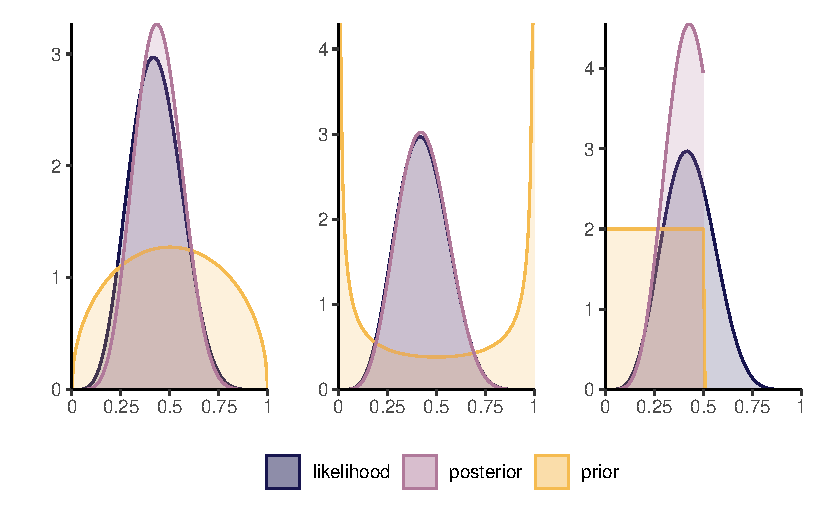
\includegraphics{introduction_files/figure-pdf/fig-betabinom-1.pdf}

}

\caption{\label{fig-betabinom}Scaled binomial likelihood for six
successes out of 14 trials, with \(\mathsf{Beta}(3/2, 3/2)\) prior
(left), \(\mathsf{Beta}(1/4, 1/4)\) (middle) and truncated uniform on
\([0,1/2]\) (right), with the corresponding posterior distributions.}

\end{figure}

\end{example}

\begin{remark}[Proportionality]

Any term appearing in the likelihood times prior function that does not
depend on parameters can be omitted since they will be absorbed by the
normalizing constant. This makes it useful to compute normalizing
constants or likelihood ratios.

\end{remark}

\begin{remark}

An alternative parametrization for the beta distribution sets
\(\alpha=\mu \kappa\), \(\beta = (1-\mu)\kappa\) for \(\mu \in (0,1)\)
and \(\kappa>0\), so that the model is parametrized directly in terms of
mean \(\mu\), with \(\kappa\) capturing the dispersion.

\end{remark}

\begin{remark}

A density integrates to 1 over the range of possible outcomes, but there
is no guarantee that the likelihood function, as a function of
\(\boldsymbol{\theta}\), integrates to one over the parameter domain
\(\boldsymbol{\Theta}\).

For example, the binomial likelihood with \(n\) trials and \(k\)
successes satisfies
\[\int_0^1 \binom{n}{k}p^k(1-p)^{n-k} \mathrm{d} p = \frac{1}{n+1}.\]

Moreover, the binomial distribution is discrete (supported on
\(0, \ldots, n\)), whereas the likelihood is continuous as a function of
the probability of success, as evidenced by
Figure~\ref{fig-binom-massvslik}

\begin{figure}[ht!]

{\centering 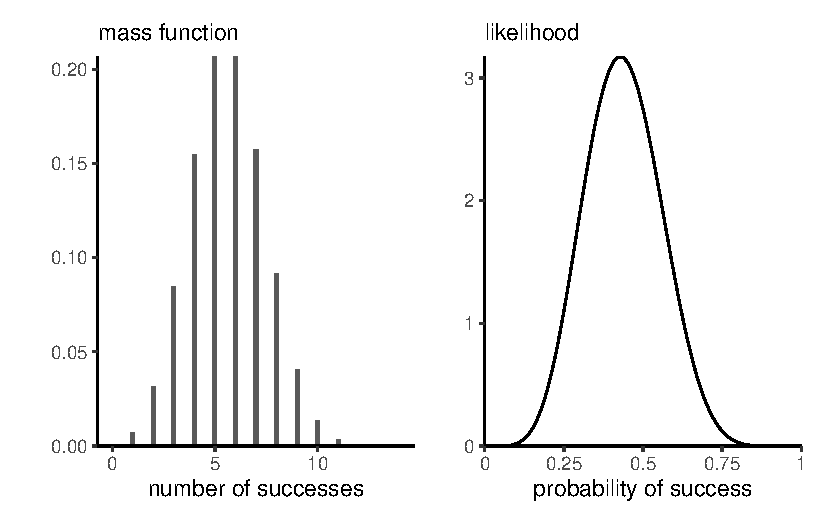
\includegraphics{introduction_files/figure-pdf/fig-binom-massvslik-1.pdf}

}

\caption{\label{fig-binom-massvslik}Binomial mass function (left) and
scaled likelihood function (right).}

\end{figure}

\end{remark}

\begin{proposition}[Sequentiality and Bayesian
updating]\protect\hypertarget{prp-sequentiality}{}\label{prp-sequentiality}

The likelihood is invariant to the order of the observations if they are
independent Thus, if we consider two blocks of observations
\(\boldsymbol{y}_1\) and \(\boldsymbol{y}_2\)
\[p(\boldsymbol{\theta} \mid \boldsymbol{y}_1, \boldsymbol{y}_2) = p(\boldsymbol{\theta} \mid \boldsymbol{y}_1) p(\boldsymbol{\theta} \mid \boldsymbol{y}_2),\]
so it makes no difference if we treat data all at once or in blocks.
More generally, for data exhibiting spatial or serial dependence, it
makes sense to consider rather the conditional (sequential)
decomposition
\[f(\boldsymbol{y}; \boldsymbol{\theta}) = f(\boldsymbol{y}_1; \boldsymbol{\theta}) f(\boldsymbol{y}_2; \boldsymbol{\theta}, \boldsymbol{y}_1) \cdots f(\boldsymbol{y}_n; \boldsymbol{\theta}, \boldsymbol{y}_1, \ldots, \boldsymbol{y}_{n-1})\]
where
\(f(\boldsymbol{y}_k; \boldsymbol{y}_1, \ldots, \boldsymbol{y}_{k-1})\)
denotes the conditional density function given observations
\(\boldsymbol{y}_1, \ldots, \boldsymbol{y}_{k-1}\).

By Bayes' rule, we can consider \emph{updating} the posterior by adding
terms to the likelihood, noting that \begin{align*}
p(\boldsymbol{\theta} \mid \boldsymbol{y}_1, \boldsymbol{y}_2) \propto p(\boldsymbol{y}_2 \mid \boldsymbol{y}_1, \boldsymbol{\theta}) p(\boldsymbol{\theta} \mid \boldsymbol{y}_1)
\end{align*} which amounts to treating the posterior
\(p(\boldsymbol{\theta} \mid \boldsymbol{y}_1)\) as a prior. If data are
exchangeable, the order in which observations are collected and the
order of the belief updating is irrelevant to the full posterior.
Figure~\ref{fig-sequential} shows how the posterior becomes gradually
closer to the scaled likelihood as we increase the sample size, and the
posterior mode moves towards the true value of the parameter (here 0.3).

\begin{figure}[ht!]

{\centering 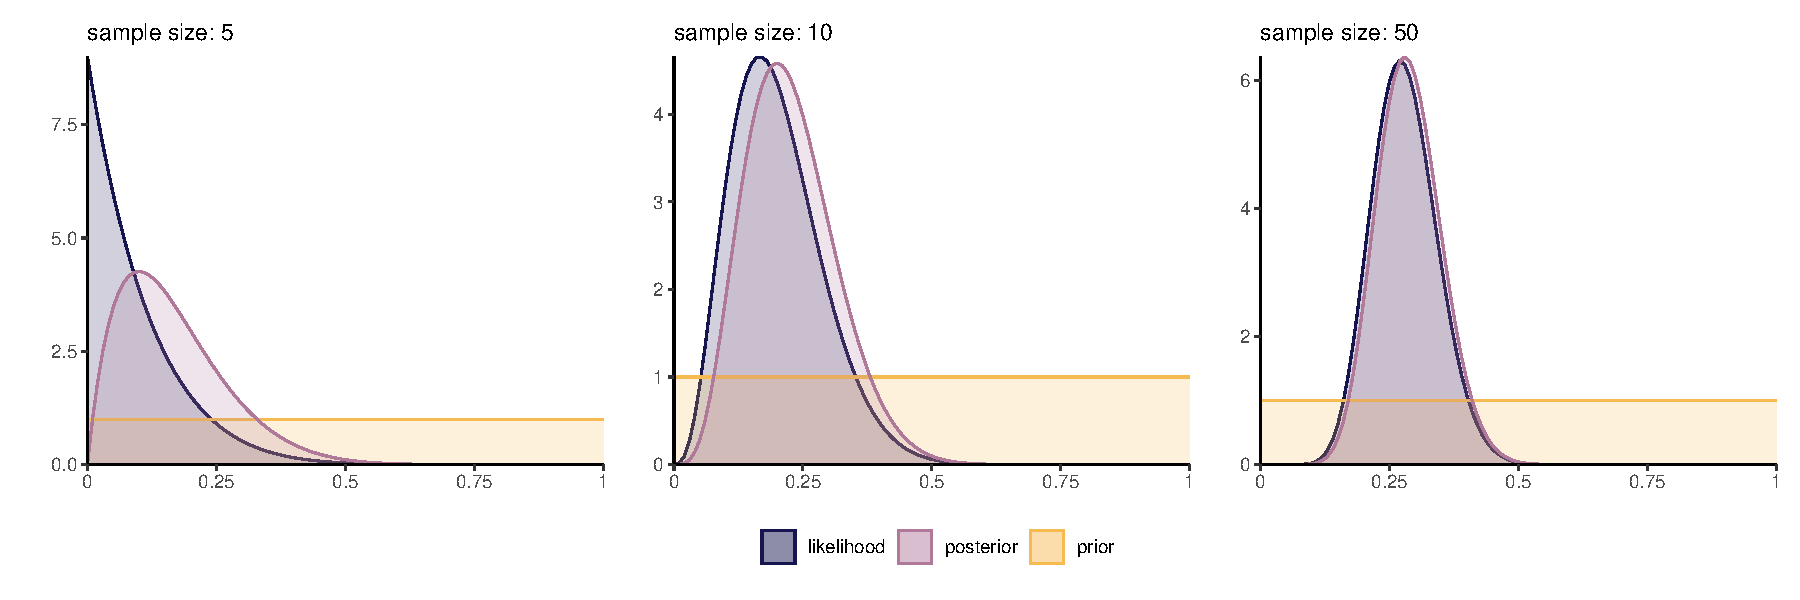
\includegraphics{introduction_files/figure-pdf/fig-sequential-1.pdf}

}

\caption{\label{fig-sequential}Beta posterior and binomial likelihood
with a uniform prior for increasing number of observations (from left to
right) out of a total of 100 trials.}

\end{figure}

\end{proposition}

\begin{example}[]\protect\hypertarget{exm-numericalintegration}{}\label{exm-numericalintegration}

While we can calculate analytically the value of the normalizing
constant for the beta-binomial model, we could also for arbitrary priors
use numerical integration or Monte Carlo methods in the event the
parameter vector \(\boldsymbol{\theta}\) is low-dimensional.

While estimation of the normalizing constant is possible in simple
models, the following highlights some challenges that are worth keeping
in mind. In a model for discrete data (that is, assigning probability
mass to a countable set of outcomes), the terms in the likelihood are
probabilities and thus the likelihood becomes smaller as we gather more
observations (since we multiply terms between zero or one). The marginal
likelihood term becomes smaller and smaller, so it's reciprocal is big
and this can lead to arithmetic underflow.

\begin{Shaded}
\begin{Highlighting}[]
\NormalTok{k }\OtherTok{\textless{}{-}}\NormalTok{ 6L }\CommentTok{\# number of successes }
\NormalTok{n }\OtherTok{\textless{}{-}}\NormalTok{ 14L }\CommentTok{\# number of trials}
\NormalTok{alpha }\OtherTok{\textless{}{-}}\NormalTok{ beta }\OtherTok{\textless{}{-}} \FloatTok{1.5} \CommentTok{\# prior parameters}
\NormalTok{unnormalized\_posterior }\OtherTok{\textless{}{-}} \ControlFlowTok{function}\NormalTok{(p)\{}
\NormalTok{  p}\SpecialCharTok{\^{}}\NormalTok{(k}\SpecialCharTok{+}\NormalTok{alpha}\DecValTok{{-}1}\NormalTok{) }\SpecialCharTok{*}\NormalTok{ (}\DecValTok{1}\SpecialCharTok{{-}}\NormalTok{p)}\SpecialCharTok{\^{}}\NormalTok{(n}\SpecialCharTok{{-}}\NormalTok{k }\SpecialCharTok{+}\NormalTok{ beta }\SpecialCharTok{{-}} \DecValTok{1}\NormalTok{)}
\NormalTok{\}}
\FunctionTok{integrate}\NormalTok{(}\AttributeTok{f =}\NormalTok{ unnormalized\_posterior,}
          \AttributeTok{lower =} \DecValTok{0}\NormalTok{,}
          \AttributeTok{upper =} \DecValTok{1}\NormalTok{)}
\end{Highlighting}
\end{Shaded}

\begin{verbatim}
1.066906e-05 with absolute error < 1e-12
\end{verbatim}

\begin{Shaded}
\begin{Highlighting}[]
\CommentTok{\# Compare with known constant}
\FunctionTok{beta}\NormalTok{(k }\SpecialCharTok{+}\NormalTok{ alpha, n }\SpecialCharTok{{-}}\NormalTok{ k }\SpecialCharTok{+}\NormalTok{ beta)}
\end{Highlighting}
\end{Shaded}

\begin{verbatim}
[1] 1.066906e-05
\end{verbatim}

\begin{Shaded}
\begin{Highlighting}[]
\CommentTok{\# Monte Carlo integration}
\FunctionTok{mean}\NormalTok{(}\FunctionTok{unnormalized\_posterior}\NormalTok{(}\FunctionTok{runif}\NormalTok{(}\FloatTok{1e5}\NormalTok{)))}
\end{Highlighting}
\end{Shaded}

\begin{verbatim}
[1] 1.064067e-05
\end{verbatim}

\end{example}

When \(\boldsymbol{\theta}\) is high-dimensional, the marginal
likelihood is intractable. This is one of the main challenges of
Bayesian statistics and the popularity and applicability has grown
drastically with the development and popularity of numerical algorithms,
following th publication of Geman and Geman
(\protect\hyperlink{ref-Geman.Geman:1984}{1984}) and Gelfand and Smith
(\protect\hyperlink{ref-Gelfand.Smith:1990}{1990}). Markov chain Monte
Carlo methods circumvent the calculation of the denominator by drawing
approximate samples from the posterior.

\hypertarget{posterior-predictive-distribution}{%
\section{Posterior predictive
distribution}\label{posterior-predictive-distribution}}

Prediction in the Bayesian paradigm is obtained by considering the
\emph{posterior predictive distribution}, \begin{align*}
p(y_{\text{new}} \mid \boldsymbol{y}) =
\int_{\Theta} p(y_{\text{new}}  \mid \boldsymbol{\theta}) p(\boldsymbol{\theta} \mid  \boldsymbol{y}) \mathrm{d} \boldsymbol{\theta}
\end{align*}

Given draws from the posterior distribution, say
\(\boldsymbol{\theta}_b\) \((b=1, \ldots, B)\), we sample from each a
new realization from the distribution appearing in the likelihood
\(p(y_{\text{new}} \mid \boldsymbol{\theta}_b)\). This is different from
the frequentist setting, which fixes the value of the parameter to some
estimate \(\widehat{\boldsymbol{\theta}}\); by contrast, the posterior
predictive, here a beta-binomial distribution
\(\mathsf{BetaBin}(n, \alpha + k, n - k + \beta)\), carries over the
uncertainty so will typically be wider and overdispersed relative to the
corresponding binomial model. This can be easily seen from the
left-panel of Figure~\ref{fig-betabinompostpred}, which contrasts the
binomial mass function evaluated at the maximum likelihood estimator
\(\widehat{p}=6/14\) with the posterior predictive.

\begin{Shaded}
\begin{Highlighting}[]
\NormalTok{npost }\OtherTok{\textless{}{-}} \FloatTok{1e4}\NormalTok{L}
\CommentTok{\# Sample draws from the posterior distribution}
\NormalTok{post\_samp }\OtherTok{\textless{}{-}} \FunctionTok{rbeta}\NormalTok{(}\AttributeTok{n =}\NormalTok{ npost, k }\SpecialCharTok{+}\NormalTok{ alpha, n }\SpecialCharTok{{-}}\NormalTok{ k }\SpecialCharTok{+}\NormalTok{ beta)}
\CommentTok{\# For each draw, sample new observation}
\NormalTok{post\_pred }\OtherTok{\textless{}{-}} \FunctionTok{rbinom}\NormalTok{(}\AttributeTok{n =}\NormalTok{ npost, }\AttributeTok{size =}\NormalTok{ n, }\AttributeTok{prob =}\NormalTok{ post\_samp)}
\end{Highlighting}
\end{Shaded}

\begin{figure}[ht!]

{\centering 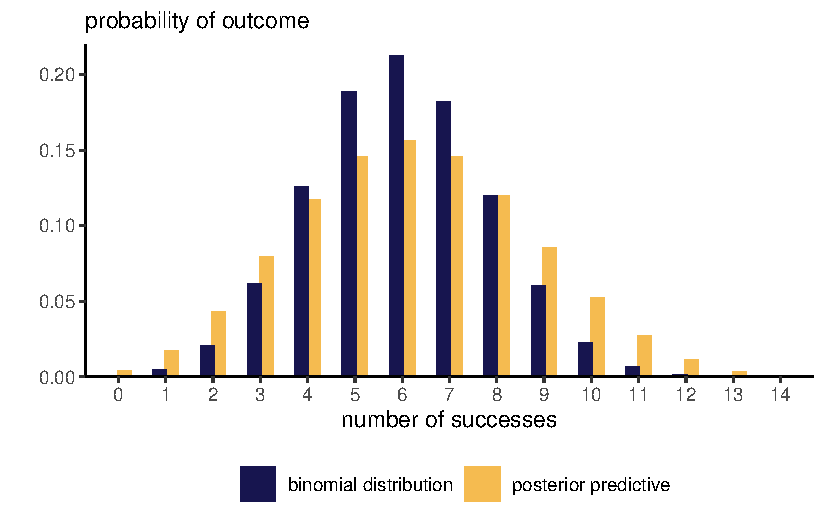
\includegraphics{introduction_files/figure-pdf/fig-betabinompostpred-1.pdf}

}

\caption{\label{fig-betabinompostpred}Beta-binomial posterior predictive
distribution with corresponding binomial mass function evaluated at the
maximum likelihood estimator.}

\end{figure}

\begin{example}[]\protect\hypertarget{exm-normal-post-pred}{}\label{exm-normal-post-pred}

Consider an \(n\) sample of independent and identically distributed
Gaussian, \(Y_i \sim \mathsf{No}(0, \tau^{-1})\) (\(i=1, \ldots, n\)),
where we assign a gamma prior on the precision
\(\tau \sim \mathsf{Ga}(\alpha, \beta)\). The posterior is
\begin{align*}
p(\tau \mid \boldsymbol{y}) \stackrel{\tau}{\propto} \prod_{i=1}^n \tau^{n/2}\exp\left(-\tau \frac{\sum_{i=1}^n{y_i^2}}{2}\right) \times \tau^{\alpha-1} \exp(-\beta \tau)
\end{align*} and rearranging the terms to collect powers of \(\tau\),
etc. we find that the posterior for \(\tau\) must also be gamma, with
shape parameter \(\alpha^* = \alpha + n/2\) and rate
\(\beta^* = \beta + \sum_{i=1}^n y_i^2/2\).

The posterior predictive is \begin{align*}
p(y_{\text{new}} \mid \boldsymbol{y}) &= \int_0^\infty \frac{\tau^{1/2}}{(2\pi)^{1/2}}\exp(-\tau y_{\text{new}}^2/2) \frac{\beta^{*\alpha^*}}{\Gamma(\alpha^*)}\tau^{\alpha^*-1}\exp(-\beta^* \tau) \mathrm{d} \tau 
\\&= (2\pi)^{-1/2} \frac{\beta^{*\alpha^*}}{\Gamma(\alpha^*)} \int_0^\infty\tau^{\alpha^*-1/2} \exp\left\{- \tau (y_{\text{new}}^2/2 + \beta^*)\right\} \mathrm{d} \tau
\\&= (2\pi)^{-1/2} \frac{\beta^{*\alpha^*}}{\Gamma(\alpha^*)} \frac{\Gamma(\alpha^* + 1/2)}{(y_{\text{new}}^2/2 + \beta^*)^{\alpha^*+1/2}}
\\&= \frac{\Gamma\left(\frac{2\alpha^* + 1}{2}\right)}{\sqrt{2\pi}\Gamma\left(\frac{2\alpha^*}{2}\right)\beta^{*1/2}} \left( 1+ \frac{y_{\text{new}}^2}{2\beta^*}\right)^{-\alpha^*-1/2}
\\&= \frac{\Gamma\left(\frac{2\alpha^* + 1}{2}\right)}{\sqrt{\pi}\sqrt{ 2\alpha^*}\Gamma\left(\frac{2\alpha^*}{2}\right)(\beta^*/\alpha^*)^{1/2}} \left( 1+ \frac{1}{2\alpha^*}\frac{y_{\text{new}}^2}{(\beta^*/\alpha^*)}\right)^{-\alpha^*-1/2}
\end{align*} which entails that \(Y_{\text{new}}\) is a scaled
Student-\(t\) distribution with scale \((\beta^*/\alpha^*)^{1/2}\) and
\(2\alpha+n\) degrees of freedom. This example also exemplifies the
additional variability relative to the distribution generating the data:
indeed, the Student-\(t\) distribution is more heavy-tailed than the
Gaussian, but since the degrees of freedom increase linearly with \(n\),
the distribution converges to a Gaussian as \(n \to \infty\), reflecting
the added information as we collect more and more data points and the
variance gets better estimated through \(\sum_{i=1}^n y_i^2/n\).

\end{example}

\hypertarget{summarizing-posterior-distributions}{%
\section{Summarizing posterior
distributions}\label{summarizing-posterior-distributions}}

Most of the field of Bayesian statistics revolves around the creation of
algorithms that either circumvent the calculation of the normalizing
constant (notably using Monte Carlo and Markov chain Monte Carlo
methods) or else provide accurate numerical approximation of the
posterior pointwise, including for marginalizing out all but one
parameters (integrated nested Laplace approximations, variational
inference, etc.) The target of inference is the whole posterior
distribution, a potentially high-dimensional object which may be
difficult to summarize or visualize. We can thus report only
characteristics of the the latter.

The choice of point summary to keep has it's root in decision theory.

\begin{definition}[Loss
function]\protect\hypertarget{def-lossfunction}{}\label{def-lossfunction}

A loss function \(c(\boldsymbol{\theta}, \boldsymbol{\upsilon})\) is a
mapping from \(\boldsymbol{\Theta} \to \mathbb{R}^k\) that assigns a
weight to each value of \(\theta\), corresponding to the regret or loss
arising from choosing this value. The corresponding point estimator
\(\widehat{\boldsymbol{\upsilon}}\) is the minimizer of the expected
loss,

\[\widehat{\boldsymbol{\upsilon}} = \mathop{\mathrm{argmin}}_{\boldsymbol{\upsilon}} \int_{\boldsymbol{\Theta}} c(\boldsymbol{\theta}, \boldsymbol{\upsilon})p(\boldsymbol{\theta} \mid \boldsymbol{y}) \mathrm{d} \boldsymbol{\theta}\]

\end{definition}

For example, in a univariate setting, the quadratic loss
\(c(\theta, \upsilon) = (\theta-\upsilon)^2\) returns the posterior
mean, the absolute loss \(c(\theta, \upsilon)=|\theta - \upsilon|\)
returns the posterior median and the 0-1 loss
\(c(\theta, \upsilon) = \mathrm{I}(\upsilon \neq \theta)\) returns the
posterior mode. All of these point estimators are central tendency
measures, but some may be more adequate depending on the setting as they
can correspond to potentially different values, as shown in the
left-panel of Figure~\ref{fig-central-moments}. The choice is
application specific: for multimodal distributions, the mode is likely a
better choice.

If we know how to evaluate the distribution numerically, we can optimize
to find the mode or else return the value for the pointwise evaluation
on a grid at which the density achieves it's maximum. The mean and
median would have to be evaluated by numerical integration if there is
no closed-form expression for the latter.

If we have rather a sample from the posterior with associated posterior
density values, then we can obtain the mode as the parameter combination
with the highest posterior, the median from the value at rank
\(\lfloor n/2\rfloor\) and the mean through the sample mean of posterior
draws.

\begin{figure}[ht!]

{\centering 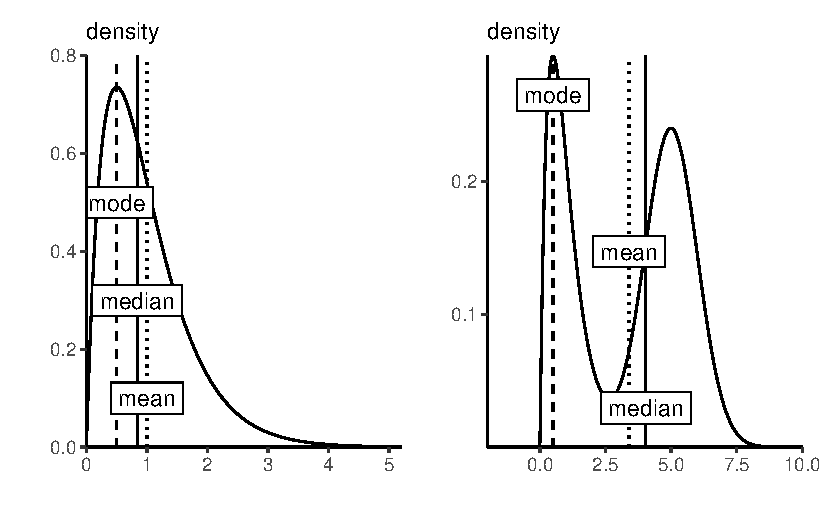
\includegraphics{introduction_files/figure-pdf/fig-central-moments-1.pdf}

}

\caption{\label{fig-central-moments}Point estimators from a left-skewed
distribution (left) and from a multimodal distribution (right).}

\end{figure}

The loss function is often a functional (meaning a one-dimensional
summary) from the posterior. The following example shows how it reduces
a three-dimensional problem into a single risk measure.

\begin{example}[]\protect\hypertarget{exm-loss-extremes}{}\label{exm-loss-extremes}

In extreme value, we are often interested in assessing the risk of
events that are rare enough that they lie beyond the range of observed
data. To provide a scientific extrapolation, it often is justified to
fit a generalized Pareto distribution to exceedances of \(Z=Y-u\), for
some user-specified threshold \(u\) which is often taken as a large
quantile of the distribution of \(Y\). The generalized Pareto
distribution function is \begin{align*}
F(z; \tau, \xi) = 1- \begin{cases}
\left(1+\xi/\tau z\right)^{-1/\xi}_{+}, & \xi \neq 0\\
\exp(-z/\tau), & \xi = 0. \end{cases}
\end{align*} The shape \(\xi\) governs how heavy-tailed the distribution
is, while \(\tau\) is a scale parameter.

Insurance companies provide coverage in exchange for premiums, but need
to safeguard themselves against very high claims by buying reinsurance
products. These risks are often communicated through the value-at-risk
(VaR), a high quantile exceeded with probability \(p\). We model Danish
fire insurance claim amounts for inflation-adjusted data collected from
January 1980 until December 1990 that are in excess of a million Danish
kroner, found in the \texttt{evir} package and analyzed in Example 7.23
of McNeil, Frey, and Embrechts
(\protect\hyperlink{ref-McNeil.Frey.Embrechts:2005}{2005}). These claims
are denoted \(Y\) and there are 2167 observations.

We fit a generalized Pareto distribution to exceedances above 10
millions krones, keeping 109 observations or roughly the largest 5\% of
the original sample. Preliminary analysis shows that we can treat data
as roughly independent and identically distributed and goodness-of-fit
diagnostics (not shown) for the generalized Pareto suggest that the fit
is adequate for all but the three largest observations, which are
(somewhat severely) underestimated by the model.

The generalized Pareto model only describes the \(n_u\) exceedances
above \(u=10\), so we need to incorporate in the likelihood a binomial
contribution for the probability \(\zeta_u\) of exceeding the threshold
\(u\). Provided that the priors for \((\tau, \xi)\) are independent of
those for \(\zeta_u\), the posterior also factorizes as a product, so
\(\zeta_u\) and \((\tau, \xi)\) are a posteriori independent.

Suppose for now that we set a \(\mathsf{Be}(0.5, 0.5)\) prior for
\(\zeta_u\) and a non-informative prior for the generalized Pareto
parameters. The \texttt{post\_samp} matrix contains exact samples from
the posterior distribution of \((\tau, \xi, \zeta_u)\), obtained using a
Monte Carlo algorithm. Our aim is to evaluate the posterior distribution
for the value-at-risk, the \(\alpha\) quantile of \(Y\) for high values
of \(\alpha\) and see what point estimator one would obtain depending on
our choice of loss function. For any \(\alpha > 1-\zeta_u\), the
\(q_{\alpha}\) is \begin{align*}
1- \alpha  &= \Pr(Y > q_\alpha \mid Y > u) \Pr(Y > u) 
\\ &= \left(1+\xi \frac{q_{\alpha}-u}{\tau}\right)_{+}^{-1/\xi}\zeta_u
\end{align*} and solving for \(q_{\alpha}\) gives \begin{align*}
q_{\alpha} = u+ \frac{\tau}{\xi} \left\{\left(\frac{\zeta_u}{1-\alpha}\right)^\xi-1\right\}.
\end{align*}

To obtain the posterior distribution of the \(\alpha\) quantile,
\(q_{\alpha}\), it suffices to plug in each posterior sample and
evaluate the function: the uncertainty is carried over from the
simulated values of the parameters to those of the quantile
\(q_{\alpha}\). The left panel of Figure~\ref{fig-lossfn} shows the
posterior density estimate of the \(\mathsf{VaR}(0.99)\) along with the
maximum a posteriori (mode) of the latter.

Suppose that we prefer to under-estimate the value-at-risk rather than
overestimate: this could be captured by the custom loss function
\begin{align*}
c(q, q_0) = 
\begin{cases}
0.5(0.99q - q_0), & q > q_0 \\
0.75(q_0 - 1.01q), & q < q_0.
\end{cases}
\end{align*} For a given value of the value-at-risk \(q_0\) evaluated on
a grid, we thus compute \begin{align*}
 r(q_0) = \int_{\boldsymbol{\Theta}}c(q(\boldsymbol{\theta}), q_0) p (\boldsymbol{\theta} \mid \boldsymbol{y}) \mathrm{d} \boldsymbol{\theta}
\end{align*} and we seek to minimize the risk,
\(\widehat{q} =\mathrm{argmin}_{q_0 \in \mathbb{R}_{+}} r(q_0)\). The
value returned that minimizes the loss, shown in
Figure~\ref{fig-lossfn}, is to the left of the posterior mean for
\(q_\alpha\).

\begin{Shaded}
\begin{Highlighting}[]
\CommentTok{\# Compute value at risk from generalized Pareto distribution quantile fn}
\NormalTok{VaR\_post }\OtherTok{\textless{}{-}} \FunctionTok{with}\NormalTok{(post\_samp,   }\CommentTok{\# data frame of posterior draws}
\NormalTok{            revdbayes}\SpecialCharTok{::}\FunctionTok{qgp}\NormalTok{(   }\CommentTok{\# with columns \textquotesingle{}probexc\textquotesingle{}, \textquotesingle{}scale\textquotesingle{}, \textquotesingle{}shape\textquotesingle{}}
  \AttributeTok{p =} \FloatTok{0.01}\SpecialCharTok{/}\NormalTok{probexc, }
  \AttributeTok{loc =} \DecValTok{10}\NormalTok{, }
  \AttributeTok{scale =}\NormalTok{ scale, }
  \AttributeTok{shape =}\NormalTok{ shape, }
  \AttributeTok{lower.tail =} \ConstantTok{FALSE}\NormalTok{))}
\CommentTok{\# Loss function}
\NormalTok{loss }\OtherTok{\textless{}{-}} \ControlFlowTok{function}\NormalTok{(qhat, q)\{}
    \FunctionTok{mean}\NormalTok{(}\FunctionTok{ifelse}\NormalTok{(q }\SpecialCharTok{\textgreater{}}\NormalTok{ qhat,}
           \FloatTok{0.5}\SpecialCharTok{*}\NormalTok{(}\FloatTok{0.99}\SpecialCharTok{*}\NormalTok{q}\SpecialCharTok{{-}}\NormalTok{qhat),}
           \FloatTok{0.75}\SpecialCharTok{*}\NormalTok{(qhat}\FloatTok{{-}1.01}\SpecialCharTok{*}\NormalTok{q)))}
\NormalTok{\}}
\CommentTok{\# Create a grid of values over which to estimate the loss for VaR}
\NormalTok{nvals }\OtherTok{\textless{}{-}}\NormalTok{ 101L}
\NormalTok{VaR\_grid }\OtherTok{\textless{}{-}} \FunctionTok{seq}\NormalTok{(}
  \AttributeTok{from =} \FunctionTok{quantile}\NormalTok{(VaR\_post, }\FloatTok{0.01}\NormalTok{),}
  \AttributeTok{to =} \FunctionTok{quantile}\NormalTok{(VaR\_post, }\FloatTok{0.99}\NormalTok{), }
  \AttributeTok{length.out =}\NormalTok{ nvals)}
\CommentTok{\# Create a container to store results}
\NormalTok{risk }\OtherTok{\textless{}{-}} \FunctionTok{numeric}\NormalTok{(}\AttributeTok{length =}\NormalTok{ nvals)}
\ControlFlowTok{for}\NormalTok{(i }\ControlFlowTok{in} \FunctionTok{seq\_len}\NormalTok{(nvals))\{}
  \CommentTok{\# Compute integral (Monte Carlo average over draws)}
\NormalTok{ risk[i] }\OtherTok{\textless{}{-}} \FunctionTok{loss}\NormalTok{(}\AttributeTok{q =}\NormalTok{ VaR\_post, }\AttributeTok{qhat =}\NormalTok{ VaR\_grid[i])}
\NormalTok{\}}
\end{Highlighting}
\end{Shaded}

\begin{figure}[ht!]

{\centering 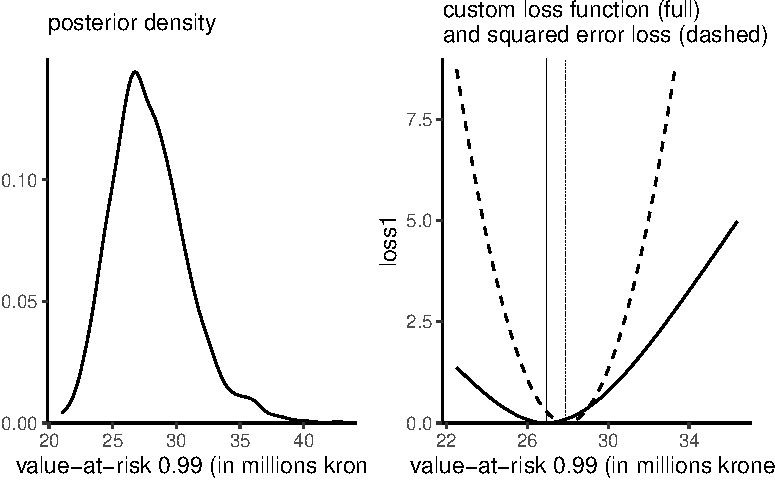
\includegraphics{introduction_files/figure-pdf/fig-lossfn-1.pdf}

}

\caption{\label{fig-lossfn}Posterior density (left) and losses
functionsfor the 0.99 value-at-risk for the Danish fire insurance data.
The vertical lines denote point estimates of the quantiles that minimize
the loss functions.}

\end{figure}

\end{example}

The output of the Bayesian learning problem will be either of:

\begin{enumerate}
\def\labelenumi{\arabic{enumi}.}
\tightlist
\item
  a fully characterized distribution
\item
  a numerical approximation to the posterior distribution (pointwise)
\item
  an exact or approximate sample drawn from the posterior distribution
\end{enumerate}

In the first case, we will be able to directly evaluate quantities of
interest if there are closed-form expressions for the latter, or else we
could draw samples from the distribution and evaluate them via
Monte-Carlo. In case of numerical approximations, we will need to resort
to numerical integration or otherwise to get our answers.

Often, we will also be interested in the marginal posterior distribution
of each component \(\theta_j\) in turn (\(j=1, \ldots, p\)). To get
these, we carry out additional integration steps,
\[p(\theta_j \mid \boldsymbol{y}) = \int p(\boldsymbol{\theta} \mid \boldsymbol{y}) \mathrm{d} \boldsymbol{\theta}_{-j}.\]
With a posterior sample, this is trivial: it suffices to keep the column
corresponding to \(\theta_j\) and discard the others.

To communicate uncertainty, we may resort to credible regions and
intervals.

\begin{definition}[]\protect\hypertarget{def-credible-region}{}\label{def-credible-region}

A \((1-\alpha)\) \textbf{credible region} (or credible interval in the
univariate setting) is a set \(\mathcal{S}_\alpha\) such that, with
probability level \(\alpha\), \begin{align*}
\Pr(\boldsymbol{\theta} \in \mathcal{S}_\alpha \mid \boldsymbol{Y}=\boldsymbol{y}) = 1-\alpha
\end{align*}

\end{definition}

These intervals are not unique, as are confidence sets. In the
univariate setting, the central or equi-tailed interval are the most
popular, and easily obtained by considering the \(\alpha/2, 1-\alpha/2\)
quantiles. These are easily obtained from samples by simply taking
empirical quantiles. An alternative, highest posterior density credible
sets, which may be a set of disjoint intervals obtained by considering
the parts of the posterior with the highest density, may be more
informative. The top panel Figure~\ref{fig-credible-intervals} shows the
distinction for a bimodal mixture distribution, and a even more striking
difference for 50\% credible intervals for a symmetric beta distribution
whose mass lie near the endpoints of the distribution, leading to no
overlap between the two intervals.

\begin{figure}[ht!]

{\centering 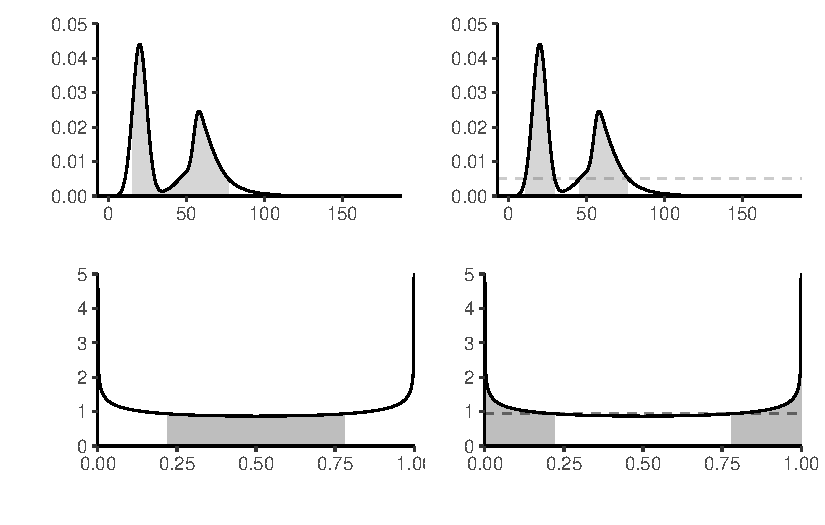
\includegraphics{introduction_files/figure-pdf/fig-credible-intervals-1.pdf}

}

\caption{\label{fig-credible-intervals}Density plots with 89\% (top) and
50\% (bottom) equitailed or central credible (left) and highest
posterior density (right) intervals for two data sets, highlighted in
grey.}

\end{figure}

Another example where these would differ

\bookmarksetup{startatroot}

\hypertarget{priors}{%
\chapter{Priors}\label{priors}}

The posterior distribution combines two ingredients: the likelihood and
the prior. If the former is a standard ingredient of any
likelihood-based inference, prior specification requires some care. The
purpose of this chapter is to consider different standard way of
constructing prior functions.

\hypertarget{conjugate-priors}{%
\section{Conjugate priors}\label{conjugate-priors}}

A distribution belongs to an exponential family with parameter vector
\(\boldsymbol{\theta} \in \mathbb{R}^D\) if it can be written as
\begin{align*}
f(y; \boldsymbol{\theta}) = \exp\left\{ \sum_{k=1}^K Q_k(\boldsymbol{\theta}) t_k(y) + D(\boldsymbol{\theta})\right\}
\end{align*} and in particular, the support does not depend on unknown
parameters. If we have an independent and identically distributed sample
of observations \(y_1, \ldots, y_n\), the log likelihood is thus of the
form \begin{align*}
\ell(\boldsymbol{\theta}) = \sum_{k=1}^K \phi_k(\boldsymbol{\theta}) \sum_{i=1}^n t_k(y_i) + n D(\boldsymbol{\theta}),
\end{align*} where the collection \(\sum_{i=1}^n t_k(y_i)\)
(\(k=1, \ldots, K\)) are sufficient statistics and
\(\phi_k(\boldsymbol{\theta})\) are the canonical parameters. The number
of sufficient statistics are the same regardless of the sample size.
Exponential families play a prominent role in generalized linear models,
in which the natural parameters are modelled as linear function of
explanatories.

A log prior density that is proportional to \begin{align*}
\log p(\boldsymbol{\theta}) \propto \eta D(\boldsymbol{\theta}) + \sum_{k=1}^K Q_k(\boldsymbol{\theta}) \nu_k
\end{align*} is conjugate.

\begin{example}[Conjugate priors for the binomial
model]\protect\hypertarget{exm-conjugatepriors-binom}{}\label{exm-conjugatepriors-binom}

The binomial log density with \(y\) successes out of \(n\) trials is
proportional to \begin{align*}
y \log(p) + (n-y) \log(1-p) = y\log\left( \frac{p}{1-p}\right) + n \log(1-p)
\end{align*} with canonical parameter \(\mathrm{logit}(p)\), which is
the natural link function for Bernoulli, giving rise to logistic
regression model. The binomial distribution is thus an exponential
family.

Since the density of the binomial is of the form \(p^y(1-p)^{n-y}\), the
beta distribution \(\mathsf{Be}(\alpha, \beta)\) with density
\[f(x) \propto x^{\alpha-1} (1-x)^{\beta-1}\] is the conjugate prior.

\end{example}

\begin{example}[Conjugate prior for the Poisson
model]\protect\hypertarget{exm-conjugatepriors-poisson}{}\label{exm-conjugatepriors-poisson}

The Poisson distribution with mean \(\mu\) has log density proportional
to \(f(y; \mu) \propto y\log(\mu) -\mu\), so is an exponential family
with natural parameter \(\log(\mu)\). The gamma density,
\[ f(x) \propto \beta^{\alpha}/\Gamma(\alpha)x^{\alpha-1} \exp(-\beta x)\]
with shape \(\alpha\) and rate \(\beta\) is the conjugate prior for the
Poisson. For an \(n\)-sample of independent observations
\(\mathsf{Po}(\mu)\) observations with
\(\mu \sim \mathsf{Ga}(\alpha, \beta)\), the posterior is
\(\mathsf{Ga}(\sum_{i=1}^n y_i + \alpha, \beta + n)\).

\end{example}

\begin{example}[Posterior rates for A/B tests using conjugate Poisson
model]\protect\hypertarget{exm-abtest}{}\label{exm-abtest}

Upworthy.com, a US media publisher, revolutionized headlines online
advertisement by running systematic A/B tests to compare the different
wording of headlines, placement and image and what catches attention the
most. The Upworthy Research Archive
(\protect\hyperlink{ref-Matias:2021}{Matias et al. 2021}) contains
results for 22743 experiments, with a click through rate of 1.58\% on
average and a standard deviation of 1.23\%. The
\texttt{clickability\_test\_id} gives the unique identifier of the
experiment, \texttt{clicks} the number of conversion out of
\texttt{impressions}. See
\href{https://tellingstorieswithdata.com/08-hunt.html\#ab-testing}{Section
8.5} of Alexander (\protect\hyperlink{ref-Alexander:2023}{2023}) for
more details about A/B testing and background information.

Consider an A/B test from November 23st, 2014, that compared four
different headlines for a story on Sesame Street workshop with
interviews of children whose parents were in jail and visiting them in
prisons. The headlines tested were:

\begin{quote}
\begin{enumerate}
\def\labelenumi{\arabic{enumi}.}
\tightlist
\item
  Some Don't Like It When He Sees His Mom. But To Him? Pure Joy. Why
  Keep Her From Him?
\item
  They're Not In Danger. They're Right. See True Compassion From The
  Children Of The Incarcerated.
\item
  Kids Have No Place In Jail \ldots{} But In This Case, They
  \emph{Totally} Deserve It.
\item
  Going To Jail \emph{Should} Be The Worst Part Of Their Life. It's So
  Not. Not At All.
\end{enumerate}
\end{quote}

At first glance, the first and third headlines seem likely to lead to a
curiosity gap. The wording of the second is more explicit (and
searchable), whereas the first is worded as a question.

We model the conversion rate \(\lambda_i\) for each headline separately
using a Poisson distribution and compare the posterior distributions for
all four choices. Using a conjugate prior and selecting the parameters
by moment matching yields approximately \(\alpha = 1.64\) and
\(\beta = 0.01\) for the hyperparameters.

\hypertarget{tbl-upworthy}{}
\begin{longtable}[]{@{}lrr@{}}
\caption{\label{tbl-upworthy}Number of views, clicks for different
headlines for the Upworthy data.}\tabularnewline
\toprule\noalign{}
headline & impressions & clicks \\
\midrule\noalign{}
\endfirsthead
\toprule\noalign{}
headline & impressions & clicks \\
\midrule\noalign{}
\endhead
\bottomrule\noalign{}
\endlastfoot
H1 & 3060 & 49 \\
H2 & 2982 & 20 \\
H3 & 3112 & 31 \\
H4 & 3083 & 9 \\
\end{longtable}

\begin{figure}[ht!]

{\centering 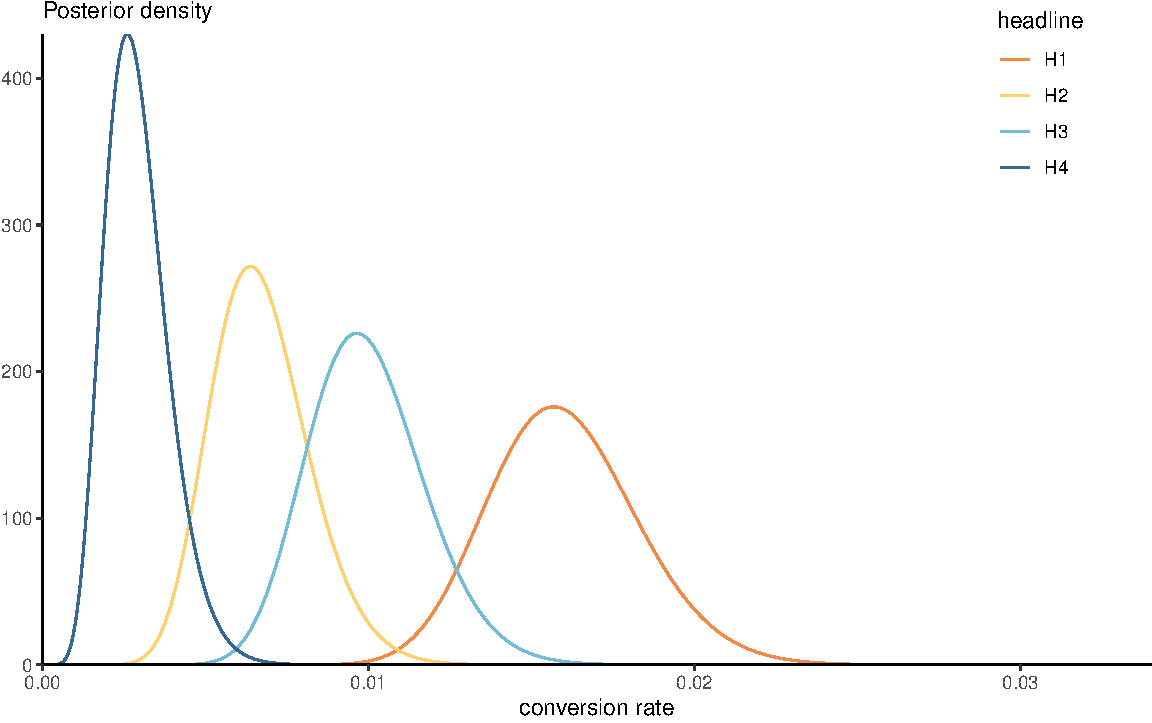
\includegraphics{priors_files/figure-pdf/fig-upworthy-1.pdf}

}

\caption{\label{fig-upworthy}Gamma posterior for the Upworthy Sesame
street headline.}

\end{figure}

We can visualize the posterior distributions. In this context, the large
sample size lead to the dominance of the likelihood contribution
\(p(Y_i \mid \lambda_i) \sim \mathsf{Po}(n_i\lambda_i)\) relative to the
prior. We can see there is virtually no overlap between different rates
for headers H1 (preferred) relative to H4 (least favorable). The
probability that Headline 3 is better than Headline 1 can be
approximated by simulating samples from both posterior and computing the
proportion of times one is larger: the probability of superiority is
1.7\%, indicating a clear preference for the first headline \texttt{H1}.

\end{example}

\begin{example}[Conjugate priors in the Bayesian linear
model]\protect\hypertarget{exm-conjugatepriors-normal}{}\label{exm-conjugatepriors-normal}

Consider a linear regression model with observation-specific mean
\(\mu_i = \mathbf{x}_i\boldsymbol{\beta}\) \((i=1,\ldots, n)\) with
\(\mathbf{x}_i\) the \(i\)th row of the \(n \times p\) design matrix
\(\mathbf{X}\).

Concatenating records,
\(\boldsymbol{Y} \sim \mathsf{No}_n(\mathbf{X}\boldsymbol{\beta}, \sigma^2 \mathbf{Q}_y^{-1})\),
for a known precision matrix \(\mathbf{Q}_y\), typically
\(\mathbf{I}_n\). To construct a conjugate joint prior for
\(p(\boldsymbol{\beta}, \sigma^2)\), we consider the sequential
formulation \begin{align*}
\boldsymbol{\beta} \mid \sigma^2 \sim \mathsf{No}_p(\boldsymbol{\nu}_\beta, \sigma^2 \mathbf{Q}^{-1}_\beta), \qquad \sigma^2 \sim \mathsf{IG}(\alpha,\beta)
\end{align*} where \(\mathsf{IG}\) denotes the inverse gamma
distribution\footnote{This simply means that the precision
  \(\sigma^{-2}\), the reciprocal of the variance, has a gamma
  distribution with shape \(\alpha\) and rate \(\beta\).}

The joint posterior is Gaussian-inverse gamma and can be factorized
\begin{align*}
p(\boldsymbol{\beta}, \sigma^2 \mid y) = p(\sigma^2 \mid y) p(\boldsymbol{\beta} \mid \sigma^2, y)
\end{align*} where
\(p(\sigma^2 \mid y) \sim \mathsf{IG}(\alpha^*, \beta^*)\) and
\(p(\boldsymbol{\beta} \mid \sigma^2, y) \sim \mathsf{No}_p(\mathbf{M}\boldsymbol{m}, \sigma^2\mathbf{M})\)
with \(\alpha^* = \alpha + n/2\),
\(\beta^*=\beta + 0.5 \boldsymbol{\nu}_\beta^\top \mathbf{Q}_\beta\boldsymbol{\nu}_\beta + \boldsymbol{y}^\top\boldsymbol{y} - \boldsymbol{m}^\top\mathbf{M}\boldsymbol{m}\),
\(\boldsymbol{m} = \mathbf{Q}_\beta \boldsymbol{\nu}_\beta + \mathbf{X}^\top \mathbf{Q}_y\boldsymbol{y}\)
and
\(\mathbf{M} = (\mathbf{Q}_\beta + \mathbf{X}^\top\mathbf{Q}_y\mathbf{X})^{-1}\);
the latter can be evaluated efficiently using
Shermann--Morrisson--Woodbury identity.

\end{example}

The exponential family is quite large;
\href{https://doi.org/10.1.1.157.5540}{Fink (1997) \emph{A Compendium of
Conjugate Priors}} gives multiple examples of conjugate priors and work
out parameter values.

One criticism of the Bayesian approach is the arbitrariness of prior
functions. However, the role of the prior is often negligible in large
samples (consider for example the posterior of exponential families with
conjugate priors). Moreover, the likelihood is also chosen for
convenience, and arguably has a bigger influence on the conclusion. Data
fitted using a linear regression model seldom follow Gaussian
distributions conditionally, in the same way that the linearity is a
convenience (and first order approximation).

In general, unless the sample size is small and we want to add expert
opinion, we may wish to pick an \emph{uninformative prior}, i.e., one
that does not impact much the outcome. For conjugate models, one can
often show that the relative weight of prior parameters (relative to the
random sample likelihood contribution) becomes negligible by
\href{https://en.wikipedia.org/wiki/Conjugate_prior}{investigating their
relative weights}.

\hypertarget{uninformative-priors}{%
\section{Uninformative priors}\label{uninformative-priors}}

\begin{definition}[Proper
prior]\protect\hypertarget{def-properprior}{}\label{def-properprior}

We call a prior \emph{proper} if it's integral is finite; such prior
function automatically leads to a valid posterior.

\end{definition}

The best example of prior priors arise from probability density
function. We can still employ this rule for improper priors: for
example, taking \(\alpha, \beta \to 0\) in the beta prior leads to a
prior proportional to \(x^{-1}(1-x)^{-1}\), the integral of which
diverges on the unit interval \([0,1]\). However, as long as the number
of success and the number of failures is larger than 1, meaning
\(k \geq 1, n-k \geq 1\), the posterior distribution would be proper,
i.e., integrable. To find the posterior, normalizing constants are also
superfluous.

Many uninformative priors are flat, or proportional to a uniform on some
subset of the real line and therefore improper. It may be superficially
tempting to set a uniform prior on a large range to ensure posterior
property, but the major problem is that a flat prior may be informative
in a different parametrization, as the following example suggests.

\begin{example}[]\protect\hypertarget{exm-scaleflatprior}{}\label{exm-scaleflatprior}

Consider the parameter \(\log(\tau) \in \mathbb{R}\) and the prior
\(p( \log \tau) \propto 1\). If we reparametrize the model in terms of
\(\tau\), the new prior (including the Jacobian of the transformation)
is \(\tau^{-1}\)

\end{example}

Some priors are standard and widely used. In location scale families
with location \(\nu\) and scale \(\tau\), the density is such that
\begin{align*}
f(x; \nu, \tau) =  \frac{1}{\tau} f\left(\frac{x - \nu}{\tau}\right), \qquad \nu \in \mathbb{R}, \tau >0.
\end{align*} We thus wish to have a prior so that
\(p(\tau) = c^{-1}p(\tau/c)\) for any scaling \(c>0\), whence it follows
that \(p(\tau) \propto \tau^{-1}\), which is uniform on the log scale.

The priors \(p(\nu) \propto 1\) and \(p(\tau) \propto \tau^{-1}\) are
both improper but lead to location and scale invariance, hence that the
result is the same regardless of the units of measurement.

\begin{definition}[Jeffrey's
prior]\protect\hypertarget{def-jeffreys}{}\label{def-jeffreys}

In single parameter models, taking a prior function for \(\theta\)
proportional to the square root of the determinant of the information
matrix \(p(\theta) \propto \imath(\theta)\) yields a prior that is
invariant to parametrization, so that inferences conducted in different
parametrizations are equivalent.\footnote{The Fisher information is
  linear in the sample size for independent and identically distributed
  data so we can derive the result for \(n=1\) without loss of
  generality.}

To see this, consider a bijective transformation
\(\theta \mapsto \vartheta\). Under the reparametrized model and
suitable regularity conditions\footnote{Using Bartlett's identity;
  Fisher consistency can be established using the dominated convergence
  theorem.}, the chain rule implies that \begin{align*}
i(\vartheta) &= - \mathsf{E} \left(\frac{\partial^2 \ell(\vartheta)}{\partial^2 \vartheta}\right)
\\&= - \mathsf{E}\left(\frac{\partial^2 \ell(\theta)}{\partial \theta^2}\right) \left( \frac{\mathrm{d} \theta}{\mathrm{d} \vartheta} \right)^2 + \mathsf{E}\left(\frac{\partial \ell(\theta)}{\partial \theta}\right) \frac{\mathrm{d}^2 \theta}{\mathrm{d} \vartheta^2}
\end{align*} Since the score has mean zero,
\(\mathsf{E}\left\{\partial \ell(\theta)/\partial \theta\right\}=0\),
the rightmost term vanishes. We can thus relate the Fisher information
in both parametrizations, with \begin{align*}
\imath^{1/2}(\vartheta) = \imath^{1/2}(\theta) \left| \frac{\mathrm{d} \theta}{\mathrm{d} \vartheta} \right|,
\end{align*} implying invariance.

Most of the times, Jeffrey's prior is improper. For the binomial model,
it can be viewed as a limiting conjugate beta prior with
\(\alpha, \beta\to 0\)). Unfortunately, in multiparameter models, the
system isn't invariant to reparametrization if we consider the
determinant of the Fisher information.

\end{definition}

\begin{example}[]\protect\hypertarget{exm-jeffreysbinom}{}\label{exm-jeffreysbinom}

Consider the binomial distribution
\(f(y; \theta, n) \propto \theta^y(1-\theta)^{n-y}\mathsf{I}_{\theta \in [0,1]}\).
The negative of the second derivative of the log likelihood with respect
to \(p\) is
\[\jmath(\theta) = - \partial^2 \ell(\theta; y) / \partial \theta^2 = y/\theta^2 + (1-y)/(1-\theta)^2\]
and since \(\mathsf{E}(Y)=n\theta\), the Fisher information is
\[\imath = \mathsf{E}\{\jmath(\theta)\}=n/\theta + n/(1-\theta) = n/\{\theta(1-\theta)\}\]
Jeffrey's prior is thus
\(p(\theta) \propto \theta^{-1}(1-\theta)^{-1}\).

\end{example}

\leavevmode\vadjust pre{\hypertarget{exer-jeffreysnormal}{}}%
Check that for the Gaussian distribution \(\mathsf{No}(\mu, \sigma^2)\),
the Jeffrey's prior obtained by treating each parameter in turn, fixing
the value of the other, are \(p(\mu) \propto 1\) and
\(p(\sigma) \propto 1/\sigma\), which also correspond to the default
uninformative priors for location-scale families.

\begin{example}[]\protect\hypertarget{exm-jeffreyspoisson}{}\label{exm-jeffreyspoisson}

The Poisson distribution with
\(\ell(\lambda) \propto -\lambda + y\log \lambda\), with second
derivative
\(-\partial^2 \ell(\lambda)/\partial \lambda^2 = y/\lambda^2\). Since
the mean of the Poisson distribution is \(\lambda\), the Fisher
information is \(\imath(\lambda) = \lambda^{-1}\) and Jeffrey's prior is
\(\lambda^{-1/2}\).

\end{example}

\hypertarget{expert-knowledge}{%
\section{Expert knowledge}\label{expert-knowledge}}

Th prior distribution may have parameters themselves that need to be
specified by experts. One may also wish to add another layer and set an
hyperprior distribution on the parameters, resulting in a hierarchical
model.

Setting parameters of priors is often done by reparametrizing the latter
in terms of moments. Sometimes, it may be easier to set priors in a
different scale where subject-matter expertise is most easily elicited.

\begin{example}[]\protect\hypertarget{exm-colestawn}{}\label{exm-colestawn}

The generalized extreme value distribution arises as the limiting
distribution for the maximum of \(m\) independent observations. The
\(\mathsf{GEV}(\mu, \sigma, \xi)\) distribution is a location-scale with
distribution function \begin{align*}
F(x) = \exp\left[ - \left\{1+\xi(x-\mu)/\sigma\right\}^{-1/\xi}_{+}\right]
\end{align*} where \(x_{+} = \max\{0, x\}\).

Inverting the distribution function yields the quantile function
\begin{align*}
Q(p) \mu + \sigma \frac{(-\log p)^{-\xi}-1}{\xi}
\end{align*}

In environmental data, we often model annual maximum. Engineering
designs are often specified in terms of the \(k\)-year return levels,
defined as the quantile of the annual maximum exceeded with probability
\(1/k\) in any given year. Using a \(\mathsf{GEV}\) for annual maximum,
Coles and Tawn (\protect\hyperlink{ref-Coles.Tawn:1996}{1996}) proposed
modelling annual daily rainfall and specifying a prior on the quantile
scale \(q_1 < q_2 < q_3\) for tail probabilities \(p_1> p_2 > p_3\). To
deal with the ordering constraints, gamma priors are imposed on the
differences \(q_1 - o \sim \mathsf{Ga}(\alpha_1, \beta_1)\),
\(q_2 - q_1 \sim \mathsf{Ga}(\alpha_2, \beta_2)\) and
\(q_3-q_2 \sim \mathsf{Ga}(\alpha_3, \beta_3)\), where \(o\) is the
lower bound of the support. The prior is thus of the form

\begin{align*}
p(\boldsymbol{q}) \propto q_1^{\alpha_1-1}\exp(-\beta_1 q_1) \prod_{i=2}^3 (q_i-q_{i-1}^{\alpha_i-1} \exp\{\beta_i(q_i-q_{i-1})\}.
\end{align*} where \(0 \leq q_1 \leq q_2 \leq q_3\). We can then relate
the prior parameters to moments.

Consider the annual maximum rainfall in Abisko, Sweden.

\end{example}

\begin{example}[Prior
simulation]\protect\hypertarget{exm-priorsim}{}\label{exm-priorsim}

Are the prior reasonable? One way to see this is to sample values from
the priors and generate new observations.

\end{example}

\begin{example}[]\protect\hypertarget{exm-priosim-gev}{}\label{exm-priosim-gev}

We can specify gamma back-transform them to location \(\mu\), scale
\(\sigma\) and shape \(\xi\) and simulate observations from the
\(\mathsf{GEV}(\mu, \sigma, \xi)\) and compare them to observations.

\end{example}

\bookmarksetup{startatroot}

\hypertarget{references}{%
\chapter*{References}\label{references}}
\addcontentsline{toc}{chapter}{References}

\markboth{References}{References}

\hypertarget{refs}{}
\begin{CSLReferences}{1}{0}
\leavevmode\vadjust pre{\hypertarget{ref-Alexander:2023}{}}%
Alexander, Rohan. 2023. \emph{Telling Stories with Data: With
Applications in {R}}. Boca Raton, FL: CRC Press.

\leavevmode\vadjust pre{\hypertarget{ref-Coles.Tawn:1996}{}}%
Coles, Stuart G., and Jonathan A. Tawn. 1996. {``A {B}ayesian Analysis
of Extreme Rainfall Data.''} \emph{Journal of the Royal Statistical
Society. Series C (Applied Statistics)} 45 (4): 463--78.
\url{https://doi.org/10.2307/2986068}.

\leavevmode\vadjust pre{\hypertarget{ref-deFinetti:1974}{}}%
Finetti, Bruno de. 1974. \emph{Theory of Probability: A Critical
Introductory Treatment}. Vol. 1. New York: Wiley.

\leavevmode\vadjust pre{\hypertarget{ref-Gelfand.Smith:1990}{}}%
Gelfand, Alan E., and Adrian F. M. Smith. 1990. {``Sampling-Based
Approaches to Calculating Marginal Densities.''} \emph{Journal of the
American Statistical Association} 85 (410): 398--409.
\url{https://doi.org/10.1080/01621459.1990.10476213}.

\leavevmode\vadjust pre{\hypertarget{ref-Geman.Geman:1984}{}}%
Geman, Stuart, and Donald Geman. 1984. {``Stochastic Relaxation, {G}ibbs
Distributions, and the {B}ayesian Restoration of Images.''} \emph{IEEE
Transactions on Pattern Analysis and Machine Intelligence} PAMI-6 (6):
721--41. \url{https://doi.org/10.1109/TPAMI.1984.4767596}.

\leavevmode\vadjust pre{\hypertarget{ref-Matias:2021}{}}%
Matias, J. Nathan, Kevin Munger, Marianne Aubin Le Quere, and Charles
Ebersole. 2021. {``The {U}pworthy {R}esearch {A}rchive, a Time Series of
32,487 Experiments in {U.S.} Media.''} \emph{Scientific Data} 8 (195).
\url{https://doi.org/10.1038/s41597-021-00934-7}.

\leavevmode\vadjust pre{\hypertarget{ref-McNeil.Frey.Embrechts:2005}{}}%
McNeil, A. J., R. Frey, and P. Embrechts. 2005. \emph{Quantitative Risk
Management: Concepts, Techniques, and Tools}. 1st ed. Princeton, NJ:
Princeton University Press.

\end{CSLReferences}


\backmatter

\end{document}
